% template d'article LaTeX créé par Max De Wilde (STIC - ULB)
% contact : madewild@ulb.ac.be

\documentclass[a4paper,12pt]{article} % ce document est un article sur une feuille A4, police taille 11

\usepackage[utf8]{inputenc} % encodé en utf-8
\usepackage[T1]{fontenc} % compatible avec les accents

\usepackage[round]{natbib} % gestion des citations
\usepackage[french]{babel} % rédigé en français
\usepackage[hyphens]{url} % formatte les liens en autorisant la césure au niveau des traits d'union
\usepackage[pdftex,urlcolor=black,colorlinks=true,linkcolor=black,citecolor=black]{hyperref} % liens cliquables mais non colorés
\usepackage[top=3cm,bottom=4cm]{geometry} % gère les marges
\usepackage{graphicx} % gestion des images
\usepackage{array} % gestion des tableaux
\usepackage{csquotes} % gestion des guillemets
\usepackage{fourier} % utilise une autre police que celle par défaut (Computer Modern)

% insérez ici d'autres extensions avec la commande \usepackage[options]{nom de l'extension}

\title{\textbf{La reconnaissance d'objets intra-images}} % le titre de l'article
\author{VANBELLE Julien} % vos prénom et nom
\date{} % pas de date

\begin{document} % début du corps du texte
\maketitle % affiche le titre, l'auteur et la date

\begin{figure}[h] % insère une figure ici (h = "here")
  \centering % centre la figure
  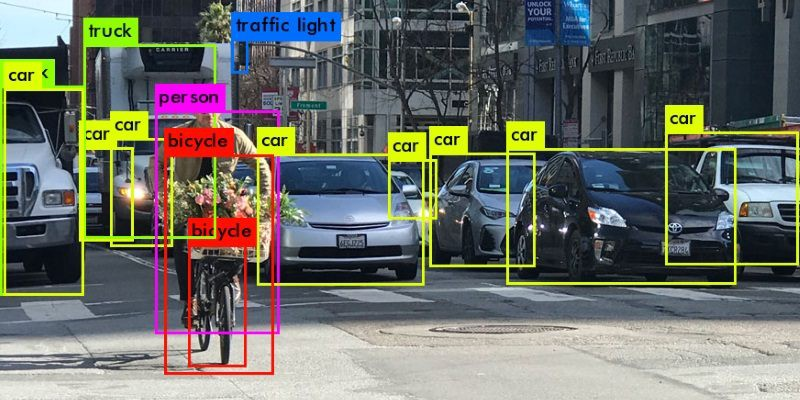
\includegraphics[scale=0.5]{illu1.jpg} % insère une image en taille réelle
  % l'extension n'est pas précisée pour éviter des problèmes de compilation
  % plus d'info ici : http://fr.wikibooks.org/wiki/LaTeX/Inclure_des_images
  \caption{\href{https://www.datagenius.fr/post/reconnaissance-d-image-intelligence-artificielle-ai-compare}{Source}} % nom de l'image
\end{figure}
\vspace{30pt}
\tableofcontents
\newpage
\section{Introduction} % section 1
		Parmi les sens présents chez l'être humain, notre vision constitue le sens le plus critique quand il s'agit d'interagir avec notre environnement. De nos jours, la quasi omniprésence du numérique amène des nouveaux défis, notamment dans la gestion numérique de l’environnement réel. Ce défi s’intitule « la vision par ordinateur » et il constituera le sujet de ce travail. \newline

	Nos interactions et notre compréhension du monde qui nous entoure repose, en autre, sur notre vision, un sens que l’on a appris à maitriser depuis notre plus jeune âge mais qui reste relativement complexe pour une machine. En effet, si nous somme capable de reconnaître en un coup d’œil un objet qui nous est familier, comment pourrais faire une machine pour nous égaler ? 
Avant de reconnaître un objet, il faut avant tout le connaître ou plutôt l’apprendre à un ordinateur. Pour cela, il faut s’intéresser à la caractérisation des objets présent dans notre environnement quotidien.  Plusieurs méthodes de caractérisation sont possibles, on pourrait définir un objet par son contour général ou par l’image de l’objet dans sa globalité ou encore via des parties de l’image de cet objet. L’ensemble de ces méthodes seront analysées dans ce travail. \newline

	En ce qui concerne la reconnaissance de ces objets caractérisés, la vision par ordinateur fait appel à différents modèles de ce que l’on caractérise aujourd’hui d’intelligence artificielle. On verra dans ce travail les limites des différentes techniques de machine learning exploitées dans le cadre de la reconnaissance d’objets. On s’intéressera notamment sur la méthode « pixels by pixels », la méthode par modèle de vecteur et les méthodes qui exploitent des réseaux de neurones.\newline

	Actuellement, les techniques de reconnaissance d’objets intra images sont exploitées dans une multitude de domaines différents, par exemple on utilise la vision par ordinateur dans le secteur des soins de santé pour identifier des tumeurs, on l’utilise aussi dans le secteur du transport pour analyser le trafic routier et permettre la genèse d’une génération de voiture autonome. L’agriculture exploite également ces techniques mais aussi le secteur de la défense pour effectuer de la reconnaissance de matériel militaire. Dès lors, on peut déduire vu la variété d’applications de ces techniques que celles-ci vont posséder une place de plus en plus prépondérante dans notre société.\newline
\newpage
\section{Principes de bases}
\textbf{1) L'image numérique }\newline
\begin{figure}[h] % insère une figure ici (h = "here")
  \centering % centre la figure
  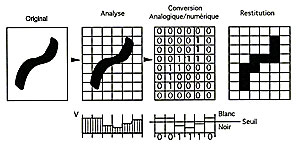
\includegraphics[scale=0.8]{binaire.jpg} % insère une image en taille réelle
  % l'extension n'est pas précisée pour éviter des problèmes de compilation
  % plus d'info ici : http://fr.wikibooks.org/wiki/LaTeX/Inclure_des_images
  \caption{\href{http://www.map.toulouse.archi.fr/works/panoformation
  /imagenum/imagenum.html}{Source} } % nom de l'image
\end{figure}
\newline
\par
	La majorité des images numériques que nous manipulons aujourd’hui sont caractérisées majoritairement par une représentation matricielle du réel. La représentation numérique d’un réel est donc un ensemble de cases appelé pixels qui restituent les informations de luminosités et de chromaticité d’un point du réel imagé. Nous ne rentrerons pas en détail ici sur le processus de captation d’une image numérique car bien que passionnant il constitue une digression dans le cadre de ce travail. \newline

	Néanmoins, il semble important de préciser une caractéristique propre à l’image numérique. En effet, celle-ci se caractérise par sa résolution que l’on pourrait simplifier par le nombre de points ou pixels que possède une image pour représenter un réel en fonction de l’unité de longueur de cette image. Cette caractéristique peut se révéler importante dans le cadre de la détection d’objets car une trop faible résolution pourrait réduire la lisibilité de la forme représentée, mais une trop grande résolution pourrait également augmenter le temps de calcul compte tenu de la quantité de détail et dès lors d’information à traiter. En effet, comme nous pourrons le constater par la suite, certain modèle de reconnaissance d’objet intra image limite les résolutions de traitement afin de conserver une efficacité optimale. \newline
 \par
    Ensuite, la synthèse des couleurs est également une caractéristique importante, car celle-ci contient des informations potentiellement importantes en ce qui concerne la caractérisation d’un objet. En effet, on distingue trois modèles de synthèses des couleurs principaux, le modèle RGB, le modèle CMJN et le modèle TSL.\newpage
\par
Le modèle RGB correspond à la synthèse additive des couleurs dans lequel un ensemble de trois couleurs primaires, le rouge, le vert et le bleu sont additionné pour former une couleur cible. Cette synthèse divise donc l’image en trois couches dans lesquelles les informations de chromaticité sont stocké est fonction des valeurs des couleurs primaires pour un pixel donné. Ce modèle est le plus couramment utilisé quand il s’agit de représentation des couleurs dans une image numérique.\newline
\par
Le modèle CMJN ou CMJK correspond quant à lui à la synthèse soustractive des couleurs. Les trois primaires cyan, magenta et jaune et le noir sont soustraite pour obtenir une couleur cible. L’image est donc décomposée en quatre composantes, une couche cyan, une couche magenta, une couche jaune et une couche comportant des informations exprimées en niveaux de gris. Ce modèle est principalement utilisé dans des fichiers numériques ayant comme finalité l’impression sur un support physique.\newline
\par
En ce qui concerne le modèle TSL, celui-ci est basé sur la modification des paramètres qui définissent une couleur. La teinte, la saturation et la luminance d’une couleur sont ainsi modifié afin d’obtenir la couleur cible désirée. Ce modèle présente une approche plus intuitive quant à la synthèse d’une couleur souhaitée mais on ne le retrouvera pas en tant que modèle d’exportation dans un fichier destiné à être visionné.\newline
\par
Dans le cadre de la reconnaissance d’objet intra-image il sera plus courant de travailler avec des images en couleurs qui utilisent la synthèse additive des couleurs correspondant au modèle RGB étant donné la prépondérance de ce modèle dans l’imagerie numérique.\newline
\newpage
\textbf{2) Reconnaissance générale et spéficique}
\newline
\par
	Dans le domaine de la vision par ordinateur, il existe deux types de reconnaissance d'objet dans une image: la reconnaissance générale et la reconnaissance spécifique. En effet, l’une va permettre de caractériser une classe d’objet alors que l’autre va s’attarder sur un objet spécifique comme c’est le cas dans le cadre de la reconnaissance faciale par exemple. 
\newline
\par
Cependant, ces deux méthodes ne font pas face aux mêmes défis. En effet, les défis de la caractérisation générale sont, par définition, moins complexe d’un point de vue pratique étant donné que ces méthodes s’arrêtent aux classes des objets. Une méthode de reconnaissance générale va caractériser l’image d’une chaise comme étant un objet chaise et non la chaise en plexiglas designé par Phillipe Starck comme on peut le voir sur les images tests ci-dessous : 
\newline
\begin{figure}[h] % insère une figure ici (h = "here")
  \centering % centre la figure
  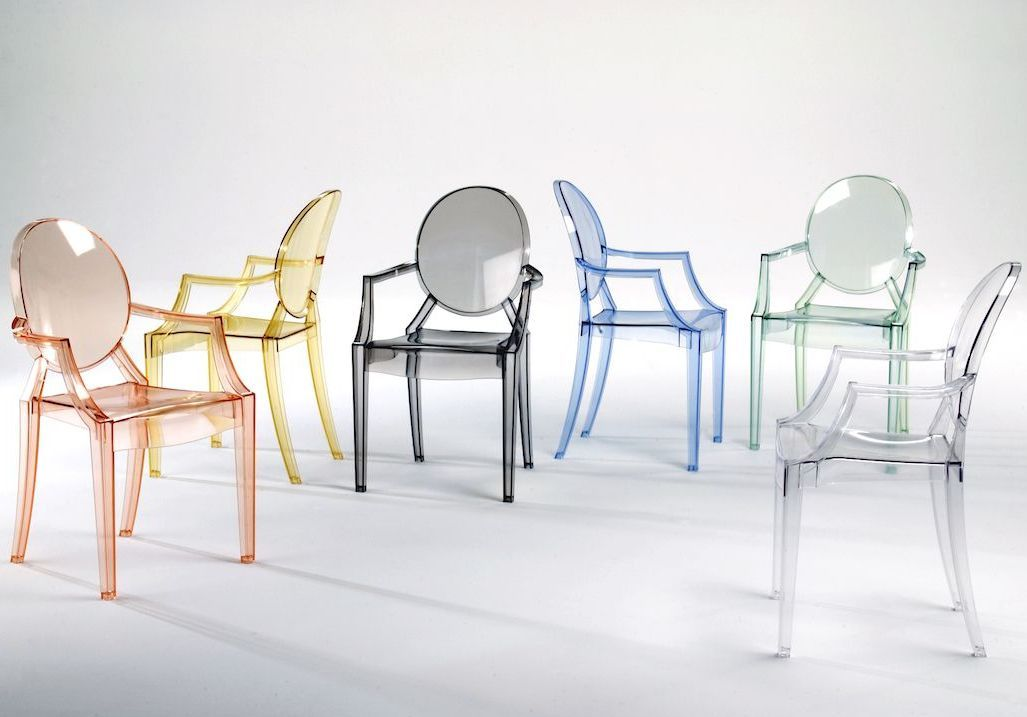
\includegraphics[scale=0.2]{stark.jpg} % insère une image en taille réelle
  % l'extension n'est pas précisée pour éviter des problèmes de compilation
  % plus d'info ici : http://fr.wikibooks.org/wiki/LaTeX/Inclure_des_images
  \caption{\href{https://www.elle.fr/Deco/Reportages/Les-pros/Philippe-Starck-le-designer-star-en-dix-realisations-iconiques}{Source} }
\end{figure}
\newline
\begin{figure}[h] % insère une figure ici (h = "here")
  \centering % centre la figure
  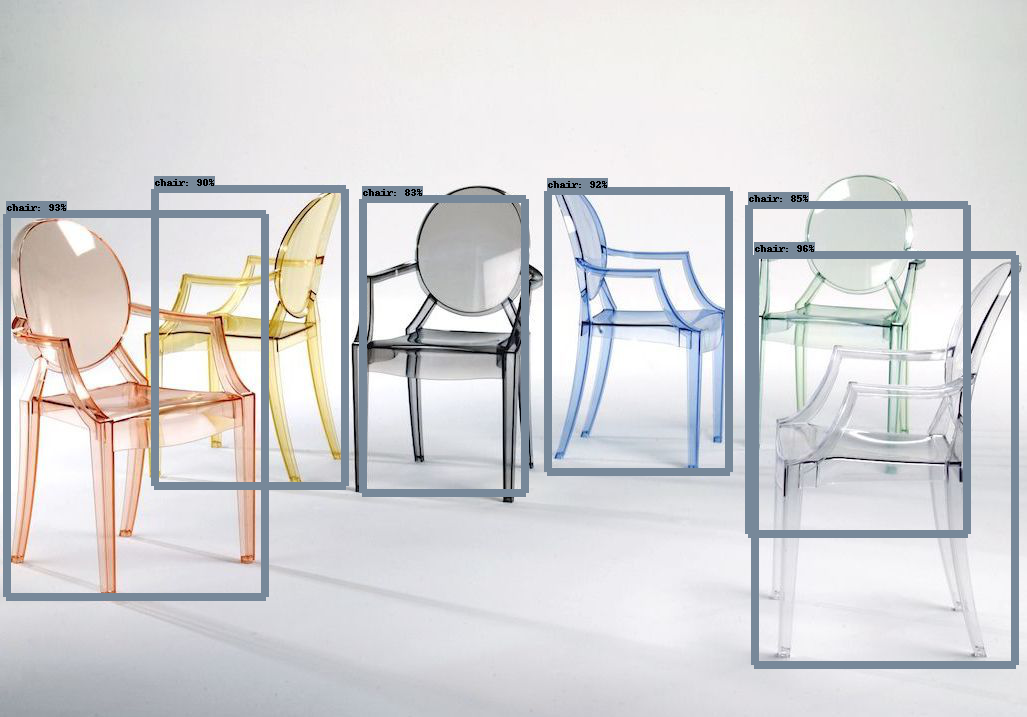
\includegraphics[scale=0.2]{output.png} % insère une image en taille réelle
  % l'extension n'est pas précisée pour éviter des problèmes de compilation
  % plus d'info ici : http://fr.wikibooks.org/wiki/LaTeX/Inclure_des_image
\end{figure}
\newpage
\par
En ce qui concerne la reconnaissance d’objet spécifique, on pourrait prendre le cas de la reconnaissance faciale. En effet, cette technologie fait partie de la reconnaissance d’objet intra images puisqu’elle passe par les mêmes procédés que la reconnaissance d’instance d’objets mais celle-ci va s’appliquer sur la singularité d’un objet de type visage. 
\newline
\par
Cette technologie ne possède pas les mêmes défis que la reconnaissance d’instance d’objets à cause de sa classification par le spécifique. Il est en effet plus complexe à faire comprendre à un ordinateur, s’il l’on prend un ensemble de chaise, laquelle de celles-ci est attribuer à quel créateur. Il faut pour permettre cela une quantité d’information bien plus conséquente dans la caractérisation d’un objet que l’on souhaite reconnaître de manière spécifique. Si l’on se penche sur la reconnaissance faciale, celle-ci fonctionne sur base de vecteurs extraits à partir des informations biométriques contenue sur le visage du sujet d’intérêt. Ces informations biométriques sont caractérisées par exemple par l’espace entre les yeux, le contour des lèvres etc… Ensuite, pour effectuer la phase de reconnaissance ces informations vectorisées sont comparées avec les informations contenue dans une base de données contenant les données acquises lors d’une phase de scanning du visage du sujet d’intérêt. 
\begin{figure}[h] % insère une figure ici (h = "here")
  \centering % centre la figure
  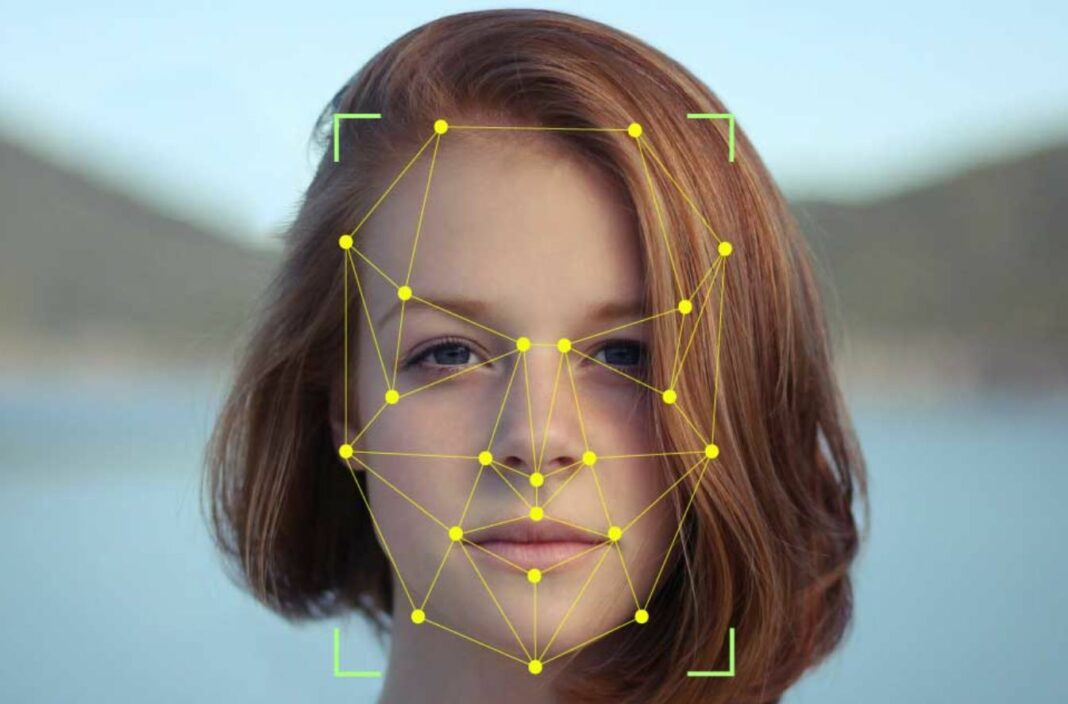
\includegraphics[scale=0.45]{face.jpg} % insère une image en taille réelle
  % l'extension n'est pas précisée pour éviter des problèmes de compilation
  % plus d'info ici : http://fr.wikibooks.org/wiki/LaTeX/Inclure_des_image
  \caption{\href{https://www.eu-startups.com/2020/12/facial-recognition-tech-risks-regulations-and-future-startup-opportunities-in-the-eu/}{Source} }
\end{figure}
\newline
\par
Dans le cadre de ce travail nous nous intéresserons principale sur la reconnaissance d’instance d’objet car le sujet de la reconnaissance spécifique pourrait se révéler un complément logique à cette première mais trop volumineux à traiter de manière détaillée dans un dossier comme celui-ci.
\newpage
\textbf{3) Les principaux défis de la reconnaissance d’instance d’objet}
\newline
\par
	La complexité de la vision par ordinateur est issue avant tout d’un problème de nature entre le monde numérique et le monde réel dans lequel nous évoluons. En effet, un ordinateur est bien plus rapide que nous lorsque qu’il s’agit de traiter des sujets a état fini que repose sur une logique prédéfinie comme un calcul mathématique par exemple, alors que l’humain lui, est extrêmement capable de travailler avec l’incertain et le changeant grâce à ses capacités cognitives et sa raison. Le défi principal de la vision par ordinateur réside donc dans cette différence de nature, il s’agit de réussir à faire comprendre un monde organique fait de singularité à une machine qui ne comprend que la logique. Si tout dans notre monde serait identique en forme et en échelle dans les images, il serait plus aisé pour un ordinateur de comparer via des correspondances mathématiques les similitudes entre deux objets. Comme cette uniformité de la représentation des objets n’est pas existante dans le monde réel, il y une série défis auxquels la vision par ordinateur devra faire face et dont voici le détail :\newline
\par

\textit{1)	Le changement de point de vue} \newline

Lorsqu’il s’agit de reconnaître un objet, le point de vue de l’on possède sur celui-ci est crucial. En effet, si notre cerveau peut reconnaître un objet de biais ou mis à l’envers, il est bien plus compliqué pour un ordinateur d’effectuer cette opération. Un objet perçu de face peut aussi être fort différent de profil et vice-versa. Il y a donc un point d’attention à considérer sur l’apparence visuelle d’un objet donné dans une situation donnée.\newline

\textit{2)	L’exposition}\newline

Le facteur d’illumination d’une image d’un objet est un élément qui peut conduire la vision par ordinateur à une confusion. L’exposition et le contraste étant lié, la modification de ce dernier peut amener un objet à être confondu avec le fond par exemple si le contraste n’est pas assez élevé. Il est donc préférable de favoriser une exposition correcte favorisant un niveau de contraste élevé pour bien discerner les différents éléments présents dans une image. \newline

\textit{3)	Le fond de l’image }\newline

Les différents éléments présents dans le fond d’une image peuvent représenter une information possible à traiter par une méthode de reconnaissance d’objet intra image ce qui amène du bruit dans l’information à traiter. En effet, une méthode de reconnaissance aura beaucoup plus facile à traiter des informations concernant un sujet sur un fond relativement vide qui isole le sujet que sur un fond contenant une multitude d’informations qui constituent des objets potentiels.\newline
\newpage
\textit{4)	Les déformations} \newline

Dans notre quotidien il existe une multitude d’objets déformable que nous reconnaissance grâce à notre appréhension des différents états de cet objet ou grâce à notre intuition. Prenons l’exemple d’une chaise pliable, dépliée elle sera reconnue par l’ordinateur comme un objet chaise mais une fois pliée celle-ci ne sera pas reconnue, bien que l’état de l’objet ait changé, sa nature est toujours la même. Il en est de même pour les objets élastiques ou possédant des morfies modifiable comme le fait notre visage en fonction de nos émotions.\newline

\textit{5)	Les occultations}\newline

Un objet est reconnu par une technique de vision par ordinateur grâce à une série de points de comparaison, dès lors si une partie de cet objet est masqué par un autre on constate une difficulté pour l’ordinateur d’effectuer une reconnaissance sur une partie tronquée d’un objet. Ceci révèle une faiblesse des systèmes actuels car compte tenu du nombre d’interactions entre objets dans notre environnement il est très complexe de les éviter. \newline

\textit{6)	Les variations intra-classe}\newline

Ce défi nait dans l’extravagance de l’esprit humain, si l’on reprend encore une fois l’exemple des chaises, on peut constater au sein de cette classe d’objet une multitude de représentation physique de l’objet chaise. Une chaise complément insolite conçue par une artiste pourrait être indiscernable par une méthode de reconnaissance d’objet alors que l’humain n’éprouverait aucune difficulté à classer l’objet artistique comme étant membre de la classe « chaise ». Cette problématique peut être directement constatée sur l'illustration ci-dessous, dans laquelle seulement trois des 12 chaises présentes ont été correctement reconnue:\newline
\begin{figure}[h] % insère une figure ici (h = "here")
  \centering % centre la figure
  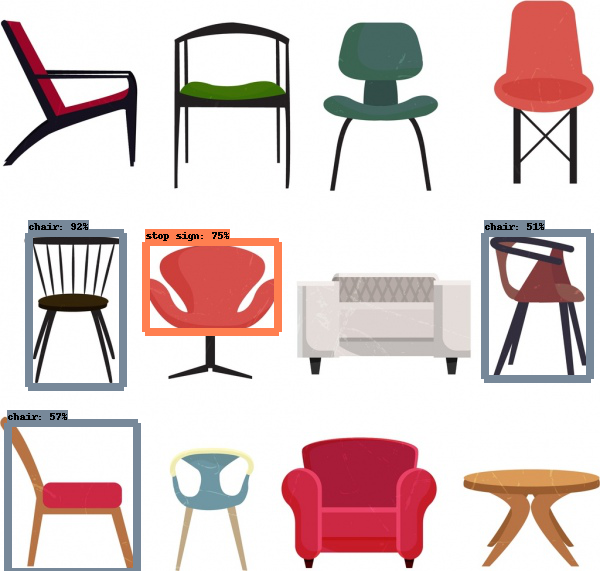
\includegraphics[scale=0.27]{chairAfterReco.png} % insère une image en taille réelle
  % l'extension n'est pas précisée pour éviter des problèmes de compilation
  % plus d'info ici : http://fr.wikibooks.org/wiki/LaTeX/Inclure_des_image
  \caption{\href{ http://gofreedownload.net/free-vector/vector-abstract/furniture-chairs-icons-collection-various-colored-types-263171/}{Source} }
\end{figure}
\newpage

\section{État de l'art} % section 2
\textbf{Bref historique}\newline
\par
	Dans la jeune histoire de reconnaissance d’objet intra image on peut constater l’apparition de plusieurs techniques au fil du temps dont voici un bref résumé :\newline

\textbf{Méthodes globales}\newline
\par
	En 2001, une première méthode de reconnaissance d’objet fait son apparition et est basée sur un procédé d’apprentissage supervisé. Cette méthode s’intitule la méthode de Viola et Jones (VJ) et elle constitue en un classifieur entrainer par des données correspondantes à l’objet cible que l’on souhaite reconnaître, une boite de détection parcoure ensuite l’entièreté de l’image pour détecter, via le contraste des pixels, la présence de l’objet cible. Cette méthode itère également sur l’image avec une échelle différente afin de ne pas discriminer les variations d’échelle. Cette méthode fut l’une des méthodes les plus considérée dans le cadre de la recherche en vision par ordinateur.\newline

\textbf{Méthodes géométriques }\newline
\par
En 2005, la méthode HOG pour « histogram of oriented gradients » fait sont apparition. Cette méthode est basée sur une décomposition de l’image en vecteurs orienté afin d’en extraire l’ensemble des formes contenues à l’intérieur de celle-ci. Comme pour la méthode VJ, celle-ci utilise un classifieur entrainé par méthode supervisée afin de fournir les données nécessaires à la reconnaissance des formes. \newline
\par
En 2008, une méthode appelée « Deformable Part Nodes » reprend la méthode de traitement de l’image HOG mais ajoute l’utilisation de SVM, de machine à vecteurs de supports pour effectuer la classification des objets présents dans l’image. La méthode SVM repose sur le principe de distance entre une frontière de séparation et les données représentées les plus proches. Cette distance est ensuite représentée sous forme de vecteurs de supports pour enfin être calculée en fonction d’une distance adéquate en fonction d’une frontière séparatrice optimale acquise à partir d’un ensemble d’apprentissage.
\newline
\par
La figure à la page suivante illustre le concept de la méthode SVM, ou l'on peut voir la frontière de séparation représentée par "hyperplane" ainsi que deux ensemble de données distincts avec deux vecteurs provenant de deux points proches de la frontière de séparation. 
\begin{figure}[h] % insère une figure ici (h = "here")
  \centering % centre la figure
  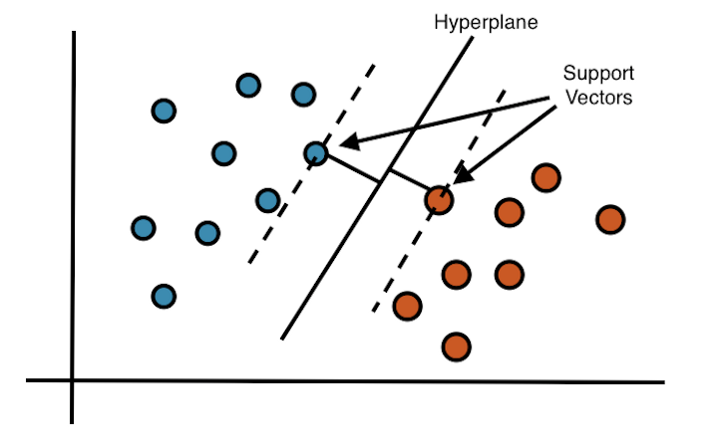
\includegraphics[scale=0.40]{vectors.png} % insère une image en taille réelle
  % l'extension n'est pas précisée pour éviter des problèmes de compilation
  % plus d'info ici : http://fr.wikibooks.org/wiki/LaTeX/Inclure_des_images
  \caption{\href{ https://ichi.pro/fr/explication-de-la-machine-vectorielle-de-support-svm-97743104690915}{Source} }
\end{figure}
\newline




\newpage
\textbf{Méthodes locales}\newline
\par
En 2013, une nouvelle méthode permet d’optimiser la recherche d’instance dans une image en se focalisant sur une analyse au préalable de l’image. En effet, lorsqu’une méthode doit balayer l’entièreté d’une image afin de rechercher d’éventuels objets celle-ci n’effectue pas un traitement optimal. Pour cela, la méthode « Selective Search » va permettre de détecter les zones de forte présence probable d’un objet afin d’y appliquer une méthode de reconnaissance donnée. \newline

\textbf{Deep learning et intelligence artificielle}\newline
\par
Entre 2012 et 2013 on verra se développer des nouvelles méthodes de reconnaissance d’objet intra-images basé sur l’utilisation de réseau de neurones et d’intelligence artificielle. Dans le cadre de ce travail nous allons nous intéresser aux réseaux de neurones de type « CNN » pour « Convolutional Neural Network » qui sont les plus utilisés dans le cadre de la vision par ordinateur.\newline
\par
Cette méthode correspondant plus à l’état de l’art actuel, elle sera détaillé dans la partie analyse de ce travail.  \newline

\newpage
\section{Analyse} % section 3}

\textbf{Artificial Neural Network et Convolutional Neural Network}\newline
\par
Dans le domaine de l’intelligence artificielle on exploite couramment des réseaux de neurones calqués sur le schéma de connections du cerveau humain. Ceux-ci sont connus sur le nom d’ « Artificial Neural Network » ou ANN et sont composés, si l’on simplifie, de 4 étapes :\newline

1)	Une étape d’entrée des données ou « input layer » qui fournit les données à la couche suivante en fonction des valeurs attribuées aux liens vers les neurones aussi appelés « weights ».\newline

2)	Une étape « cachée » ou « hidden layer » contenant les neurones artificiels. Cette couche effectue ses opérations sur base d’une méthode de propagation vers l’avant (« forward propagation). Cette méthode fonctionne grâce à un principe d’activation des neurones artificiel sur base d’une valeur minimale d’activation (« threshold »). Les données fournies à la première couche de neurones activent certains d’entre eux qui vont activer en cascade d’autre neurones connectés ensemble dans des couches suivantes.\newline

3)	Une étape de sortie ou « output layer » qui fournit le résultat des prédictions effectuées par le réseau de neurones. \newline

4)	Une étape de vérification en fonction des données apprises par l’intelligence artificielle sur base d’un entrainement préalable avec des données vérifiées. Cette étape permet de vérifier les prédictions effectuées par l’étape de sortie via une méthode appelée propagation vers l’arrière ou « backpropagation ». Cette méthode permet de calibrer le réseau de neurones en modifiant les valeurs des liens vers les neurones (« weights ») durant la phase d’apprentissage. \newline
\begin{figure}[h] % insère une figure ici (h = "here")
  \centering % centre la figure
  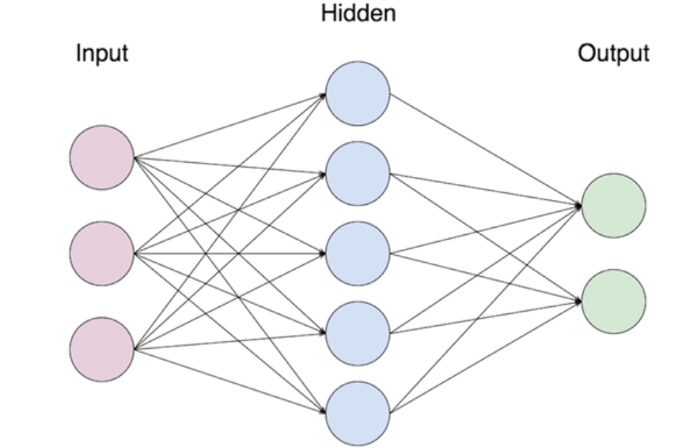
\includegraphics[scale=0.30]{ANN.png} % insère une image en taille réelle
  % l'extension n'est pas précisée pour éviter des problèmes de compilation
  % plus d'info ici : http://fr.wikibooks.org/wiki/LaTeX/Inclure_des_images
  \caption{\href{https://towardsdatascience.com/step-by-step-guide-to-building-your-own-neural-network-from-scratch-df64b1c5ab6e}{Source} }
\end{figure}
\newpage
\par
Dans le cadre de la reconnaissance d’objet, il est plus courant d’exploiter un autre type de réseau de neurones, le « Convolutional Neural Networks » ou « CNN ». Cette méthode de « deep learning » est capable d’extraire les différents points d’intérêts présent dans une image et d’en attribuer une importance relative. 
Comme pour les réseaux de neurones classiques, les CNNs sont basés sur l’arborescence du cerveau humain mais ceux-ci sont directement inspirés du fonctionnement du cortex visuel de notre cerveau. Chaque neurone présent dans le réseau répond à un stimulus actif dans une région d’intérêt définie pour celui-ci. \newline
\par
	Pour ce faire, le CNN exploite une série de filtre qui réduit une matrice de pixels définie en un vecteurs de valeurs correspondantes. Cette méthode permet de réduire considérablement la quantité de donnée à traiter pour identifier un objet dans une image. Ce type d’intelligence artificielle est particulièrement efficace pour reconnaitre des similitudes entre deux images. Elle possède également une étape d’apprentissage préalable afin d’enrichir les connaissances du classifieur utilisé après les étapes d’extractions d’informations par convolution. \newline
\par
Le procédé mis en œuvre par ce système repose sur l’utilisation d’un filtre ou matrice de convolution qui rend uniforme les calculs effectués par les neurones du réseau sur leur zone d’intérêt définie. Cependant, chaque couche composant l’image (RGB) est analysée avec un filtre différent. Les informations extraites sont ensuite synthétisées dans une matrice sur base de la réponse des neurones (Pooling). Cette étape permet de générer une version simplifiée de l’image en en retenant que l’essentiel ce qui permet d’optimiser la quantité de données à traiter. Après les étapes de covolution successives, l’ensemble des matrices de pooling obtenue sont transformées en un vecteur contenant une version en une dimension des données extraites. Ce vecteur est ensuite introduit dans un système de classification basé sur un réseau de neurone ANN FeedForward qui comme expliqué précédemment va effectuer une prédiction sur base des données acquises lors de la phase d’apprentissage. \newline
\begin{figure}[h] % insère une figure ici (h = "here")
  \centering % centre la figure
  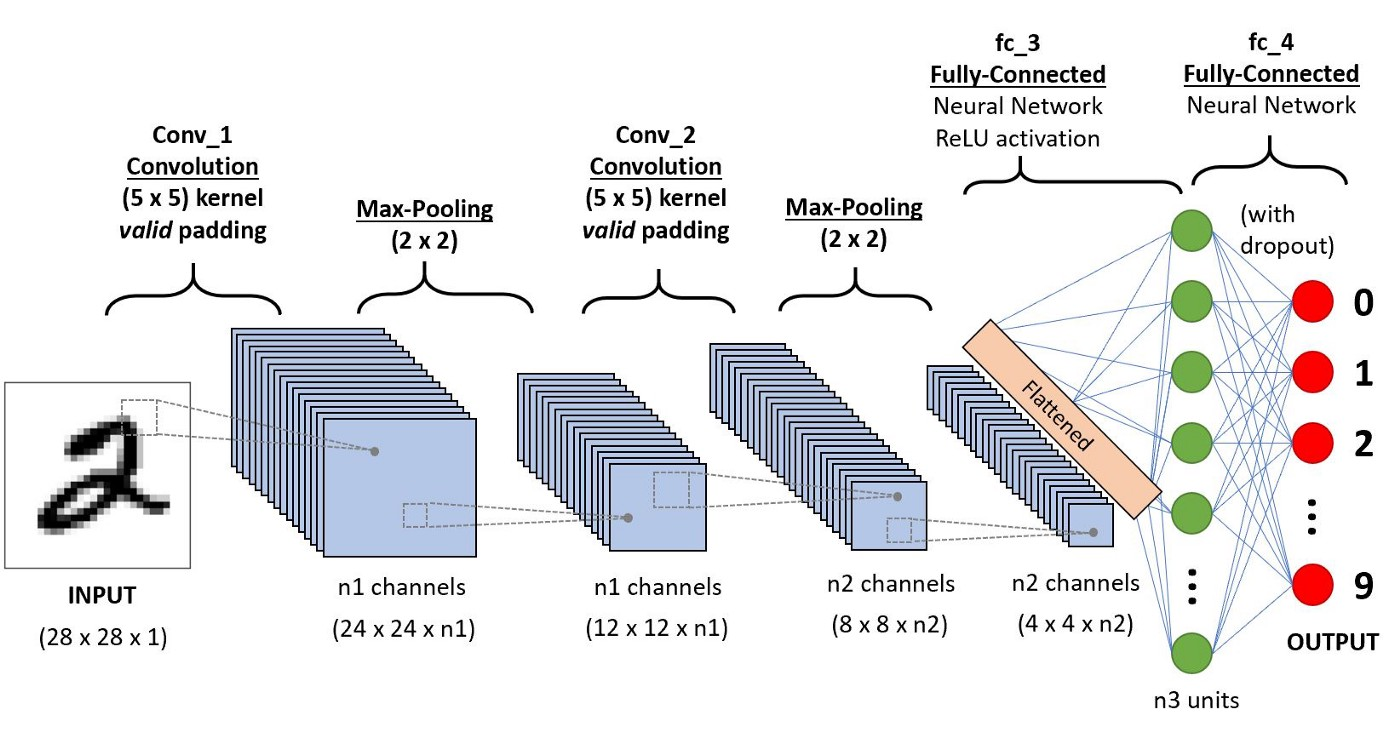
\includegraphics[scale=0.20]{CNN.jpeg} % insère une image en taille réelle
  % l'extension n'est pas précisée pour éviter des problèmes de compilation
  % plus d'info ici : http://fr.wikibooks.org/wiki/LaTeX/Inclure_des_images
  \caption{\href{https://towardsdatascience.com/a-comprehensive-guide-to-convolutional-neural-networks-the-eli5-way-3bd2b1164a53}{Source} }
\end{figure}
\newpage
\textbf{Les différentes approches basées sur le deep learning}\newline

\textit{1)	R-CNN}\newline

Les méthodes R-CNN pour « Region-based Convolutional Neural Networks » sont basées sur une approche selective qui va extraire des zones d’intérêt dans l’image afin de les fournir dans le réseau de neurones CNN. Le temps d’entrainement de cette méthode est particulièrement long puisque chaque division d’image est fournie au réseau de neurones.\newline 

\textit{2)	Fast R-CNN}\newline

Afin de palier au problème de lenteur de la méthode R-CNN, une méthode appelée « Fast R-CNN » a été introduite, celle-ci effectue une analyse globale de l’image au lieu de passer par une multitude de région d’intérêt.\newline

\textit{3)	YOLO}\newline 

La méthode « YOLO » pour « You Only Look Once” est une des méthodes les plus rapide car celle-ci utilise un seul réseau de neurones sur l’entièreté de l’image. Cette méthode repose sur un modèle d’intelligence artificielle pré-entrainé qui lui permet de discerner des formes dans l’image grâce à une navigation transversale de l’image. Cette méthode exécute aussi son analyse avec une multitude d’échelle différente pour un objet donné afin de ne pas discriminer les différences d’échelle. L’ensemble de l’analyse résulte en une liste de probabilité d’objets reconnus et l’algorithme expose l’objet correspondant à la probabilité la plus élevée.\newline
\begin{figure}[h] % insère une figure ici (h = "here")
  \centering % centre la figure
  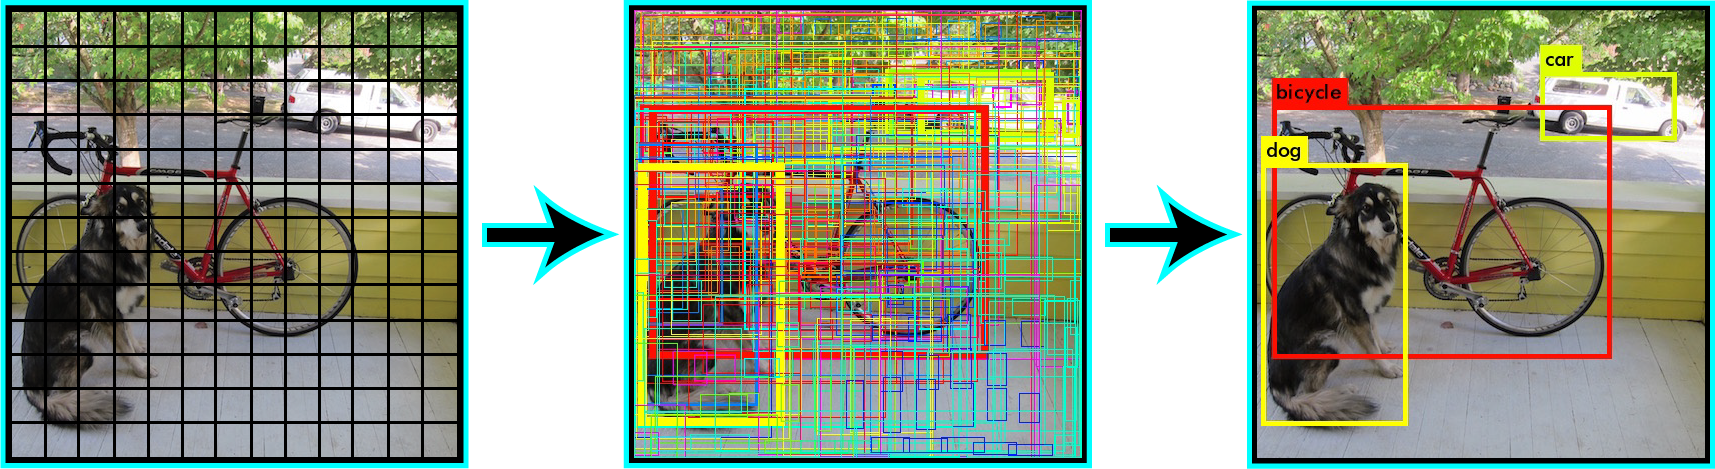
\includegraphics[scale=0.20]{YOLO.png} % insère une image en taille réelle
  % l'extension n'est pas précisée pour éviter des problèmes de compilation
  % plus d'info ici : http://fr.wikibooks.org/wiki/LaTeX/Inclure_des_images
  \caption{\href{https://pjreddie.com/darknet/yolov2/}{Source} }
\end{figure}
\newpage
\textit{4)	SSD}\newline

La méthode « SSD » ou « Single Shot Detector » est une méthode basée sur la génération de boite de détection associé à l’utilisation de réseau de neurone de type CNN au sein de l’image analysée. 
Ces boites de recherche sont générées par un algorithme qui se base sur un point d’ancrage défini par un pixel présent dans l’image analysée.  Il résulte de cette opération une multitude de boites de recherches (orientées de manière horizontale et verticale). Chacune de ces boites de recherche est ensuite analysée pour en extraire les éventuels objets présents dans l’image.\newline 
\begin{figure}[h] % insère une figure ici (h = "here")
  \centering % centre la figure
  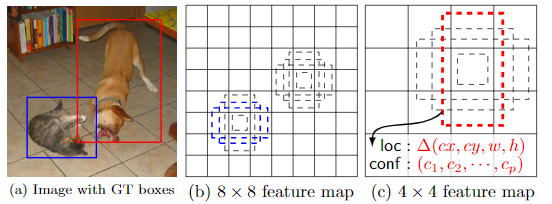
\includegraphics[scale=0.80]{ssd.png} % insère une image en taille réelle
  % l'extension n'est pas précisée pour éviter des problèmes de compilation
  % plus d'info ici : http://fr.wikibooks.org/wiki/LaTeX/Inclure_des_images
   \caption{\href{https://towardsdatascience.com/review-ssd-single-shot-detector-object-detection-851a94607d11}{Source} }
\end{figure}

\newpage
\section{Conclusion} % section 4
Parmi tous les défis du monde technologique de demain, la compréhension de notre monde et des interactions multiples est cruciale pour permettre à une machine dans nous aider dans des taches complexe. La vision par ordinateur et l’intelligence artificielle constituent dès lors des disciplines d’avenir qui ne peuvent que prendre de l’ampleur dans les années à venir. On peut déjà constater son importance dans une multitude de secteur, le secteur des transports par exemple avec son lot de véhicule autonome qui sans cette méthode de traitement de notre environnement serait tout bonnement incapable de prendre des décisions. On constate aussi l’importance de cette technologie dans le domaine des soins de santé, dans lequel la vision par ordinateur permet au personnel soignant d’identifier la sévérité de certaines tumeurs. \newline
\par
	Il est nécessaire d’appréhender cette technologie avec un certain regard critique également. En effet, si une machine peut voir et comprendre le monde, celle-ci étant pour l’instant dépourvue de raison, il est complexe d’attribuer une confiance absolue dans ses décisions. Cependant, il est important de raisonner les doutes sur l’efficacité de ces méthodes et sur les données qu’elles nous amènent à traiter. Il est donc crucial de connaître et de comprendre cette technologie et ces différentes méthodes de traitements afin de pouvoir exercer une critique active et justifié sur les données extraites grâce à la vision par ordinateur. \newline
\par
	Enfin, le couple vision par ordinateur et intelligence artificielle sont amené à nous permettre dans les années à venir à augmenter nos capacités d’analyse sur notre monde et d’optimisé celui-ci afin de le rendre plus sûr. Avec des techniques de plus en plus efficace et rapide, nous sommes déjà en mesure aujourd’hui d’effectuer de la vision par ordinateur presque en temps réel. Il en découle ainsi une série de prédictions qui dans certain cas permette d’anticiper des évènements ou des modifications d’états à venir. Gardons un œil attentif sur cette technologie qui si jeune soit elle, nous promet déjà un lot d’avancées conséquent dans l’avenir pour une multitude de secteurs cruciaux dans notre vie quotidienne. 
\newpage

\nocite {*}
\bibliographystyle{plainnat-fr} % paramètre l'affichage de la bibliographie
\bibliography{biblioVJ}
\end{document} % fin du corps du texte